\subsection{Không gian vector}
Tiếp tục đào sâu vào một khía cạnh của các khái niệm đã được nhắc tới, ta sẽ phát hiện thêm nhiều điều kỳ thú. Sau đây chính là một minh chứng.
\subsubsection*{Cơ sở}
Dựa theo định nghĩa, một hệ vector cơ sở là hệ vector sao cho mọi vector trong không gian đều có thể được phân tích thành một \emph{tổ hợp tuyến tính} của chúng. Nói cách khác, giả sử ta có hai vector cơ sở \(\mathbf{e}_i\) và \(\mathbf{e}_j\), một vector \(\mathbf{v}\) bất kỳ có thể được viết thành \[\mathbf{v}=\alpha\mathbf{e}_1 +\beta\mathbf{e}_2.\] Ta lại xét một hệ cơ sở khác gồm hai vector \(\mathbf{e}_{3}, \mathbf{e}_4\), lúc này \[\mathbf{v}=\gamma\mathbf{e}_3 +\sigma\mathbf{e}_4.\]
Một ví dụ  minh hoạ điều này:
\[\mathbf{v}= (5;3)=5(1;0)+3(0;1)=1(2;-3)
+3(1;2).\] Vector \(\mathbf{v}\) đầu tiên được phân tích thành hai vector cơ sở trực chuẩn, rồi sau đó lại được phân tích thành hai vector \[
\mathbf{e}_3 =(2;-3),\qquad \text{ và } \mathbf{e}_4 =(1;2).\] 
\begin{figure}[H]
    \centering
    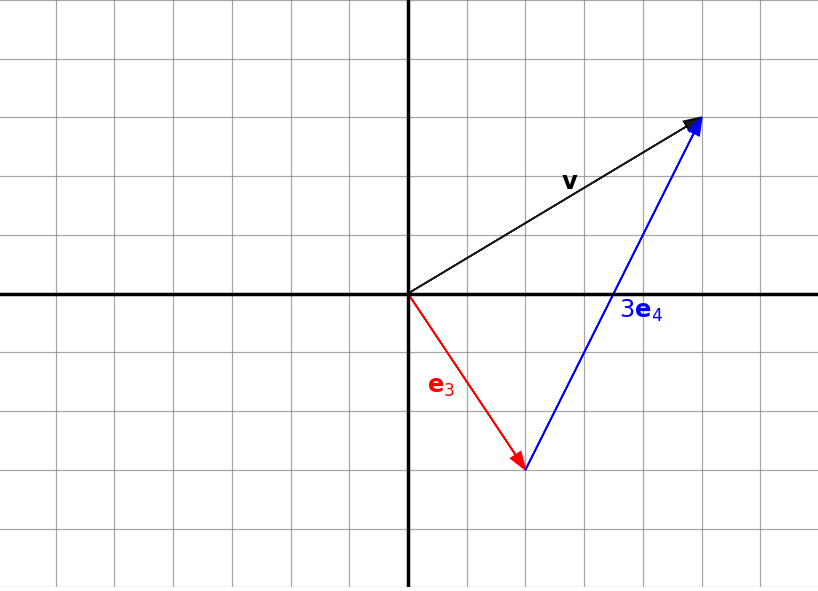
\includegraphics[width=0.6\linewidth]{Tuan2/Figures/e3e4.png}
\end{figure}
Lúc này hai vector cơ sở 3,4 không trực chuẩn và được viết trong toạ độ tạo bởi hai vector cơ sở trực chuẩn 1,2- hai vector được chọn để có toạ độ \((1,0)\) và \((0,1)\).

Một tổ hợp tuyến tính của hai vector nói rằng ta đã kéo giãn mỗi vector theo một hệ số nào đó và sau đó cộng chúng với nhau. Đặc biệt, đối với hai vector mới được chọn, bằng cách lựa chọn một bộ hệ số vô hướng thích hợp, ta có thể biểu diễn mọi vector trên mặt phẳng thành một tổ hợp tuyến tính của chúng (do đó ta chọn chúng làm cơ sở, như đã đề cập). 
Mặt khác, nếu hai vector ta chọn chỉ là \(\mathbf{e}_3\) và, chẳng hạn, \(2\mathbf{e}_3\), những vector có thể được biểu diễn bởi hệ vector (không phải cơ sở) này chỉ có những vector nằm trên cùng một đường thẳng với \(\mathbf{e}_3\). Nhưng đồng thời, nếu ta chỉ quan tâm tới 
những thứ xảy ra trên đường thẳng đó, thì bất kỳ một (và chỉ một) vector nào nằm trên đó đều là cơ sở cho \emph{không gian}(đường thẳng) mà ta quan tâm.
\begin{figure}[H]
    \centering
    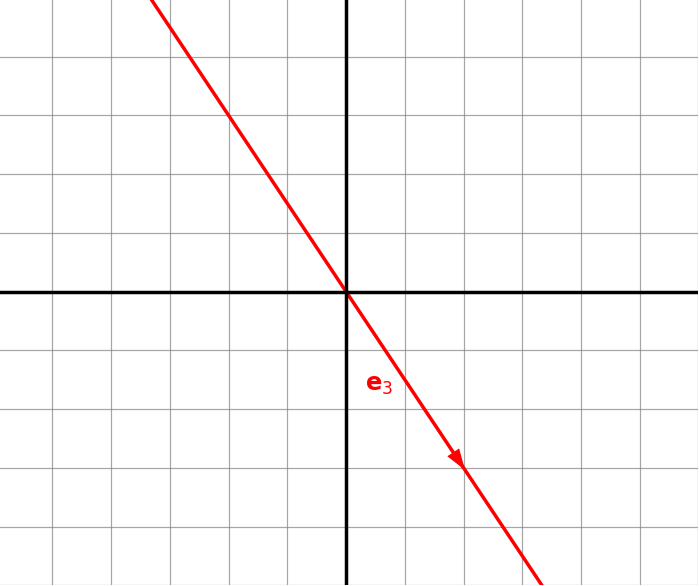
\includegraphics[width=0.6\textwidth]{Tuan2/Figures/avectoronaline.png}
\end{figure}

\vspace{8pt}

Một cách tự nhiên, ta đi tới những khái niệm sau:
\begin{definition}[Bao tuyến tính]
    Nếu \(S=\{\mathbf{u}_{1}, \mathbf{u}_{2},\dots,  \mathbf{u}_{n}\}\) là một tập hợp \(n\) vector trong không gian, thì tập hợp tất cả các tổ hợp tuyến tính của chúng được gọi là bao tuyến tính của \(\mathbf{u}_{1}, \mathbf{u}_{2},\dots \mathbf{u}_{n}\), và được kí hiệu là span(\(S\)).
    \vspace{8pt}

    Nếu span(S) chứa toàn bộ vector trong không gian, vậy ta gọi S là một hệ sinh cho không gian.
\end{definition}

\begin{definition}[Độc lập tuyến tính]
    Một tập hợp các vector được gọi là \emph{độc lập tuyến tính} với nhau nếu tổ hợp tuyến tính của chúng không bao giờ bằng \(\mathbf{0}\) trừ khi \textbf{tất cả} các hệ số vô hướng đều bằng \(0\).
\end{definition}
\begin{definition}[Hệ cơ sở]
    Một cơ sở của không gian là một tập hợp các vector trong không gian sao cho 
    \begin{itemize}
        \item tạo thành hệ sinh cho không gian, và
        \item độc lập tuyến tính.\footnote{Có thể chứng minh rằng mỗi vector trong không gian tương ứng với duy nhất một tổ hợp tuyến tính của cùng một hệ cơ sở. Đây là một bài tập cho các bạn.}
    \end{itemize}
\end{definition}
Trong ví dụ cụ thể ta đã lấy ở trên, không gian của ta (một mặt phẳng) có hai hệ sinh là \(S_1 =\{\mathbf{e}_{1}, \mathbf{e}_2\}\), và \(S_2 =\{\mathbf{e}_{3}, \mathbf{e}_{4}\}\). Đồng thời, hai cặp vector tạo thành hai hệ sinh này cũng là các cơ sở khác nhau. Ngoài ra cũng chú ý rằng, \(S_{3}=\{\mathbf{e}_{3}, \mathbf{e}_{4}, 2\mathbf{e}_{3}\}\) cũng là một hệ sinh cho mặt phẳng này nhưng tập hợp ba vector này không phải là một hệ cơ sở, vì nó không độc lập tuyến tính (phụ thuộc tuyến tính). Cụ thể, dễ thấy rằng \[-2\mathbf{e}_{3}+1(2\mathbf{e}_{3})+0\mathbf{e}_{4}=\mathbf{0},\] nhưng ta lại có các hệ số khác \(0\) là \(-2\) và \(1\). Ngoài ra, bất kỳ một tập hợp vector nào chứa vector \(\mathbf{0}\) đều không độc lập tuyến tính, và do đó không phải là một hệ cơ sở.

\subsubsection*{Không gian vector}
Khi đề cập đến vector, ta không tránh khỏi đề cập đến từ "không gian". Trong phần \ref{vector}, từ này được hiểu là không gian ba chiều mà ta sinh hoạt, có trên dưới, phải trái, trước sau; tức là không gian hình học. Song, trong phần vừa rồi, từ "không gian" được dùng một cách nhập nhằng, tối nghĩa. Thoạt đầu là nghĩa ở \ref{vector}. Rồi trong các phần định nghĩa mới được đưa ra, nó dường như cũng chỉ để chỉ mặt phẳng toạ độ Oxy, chỉ chứa các vector có hai thành phần toạ độ. Số vector cơ sở cho không gian này cũng chỉ là \(2\) mà không phải \(3\). Việc nói rằng "bởi vì vector đại diện cho trên dưới lúc này bằng \(\mathbf{0}\) nên không được xét vào" là vô nghĩa và không đúng với các định nghĩa được đưa ra. 
Thành thử, cần làm rõ nghĩa của cụm "không gian chứa các vector".
\vspace{8pt}

\begin{definition}\label{def2.2.4}
    Một không gian vector \(V\) là một tập hợp mà các phần tử trong đó, được gọi là vector thoả mãn 
    \begin{enumerate}
        \item[(i)] Với mọi \(\mathbf{v}, \mathbf{w}\in V , \mathbf{v}+\mathbf{w}\in V\).
        \item[(ii)] Với mọi \(\mathbf{v}\in V, \alpha\in \mathbb{R}, \alpha\mathbf{v}\in V\).
        \item[(iii)]  \(\mathbf{v}+\mathbf{w}=\mathbf{w}+\mathbf{v}\).
        \item[(iv)]    \(\mathbf{u}+(\mathbf{v}+\mathbf{w})=(\mathbf{u}+\mathbf{v})+\mathbf{w}\).
        \item[(v)] Tồn tại một vector \(\mathbf{0}\) sao cho \(\mathbf{v}+\mathbf{0}=\mathbf{v}\).
        \item[(vi)] Với mọi vector \(\mathbf{v}\), tồn tại một vector \(\mathbf{v}'\) sao cho \(\mathbf{v}+\mathbf{v}'=\mathbf{0}\).
        \item[(vii)] \(1\mathbf{v}=\mathbf{v}\).
        \item[(viii)] \(\alpha(\beta\mathbf{v})=(\alpha\beta)\mathbf{v}\).
        \item[(ix)]  \(\alpha(\mathbf{v}+\mathbf{w})=\alpha\mathbf{v}+\alpha\mathbf{w}\).
        \item[(x)] \((\alpha+\beta)\mathbf{v}=\alpha\mathbf{v}+\beta\mathbf{v}\).    
    \end{enumerate}
\end{definition}
Dưới góc nhìn của một tập hợp, ta quay lại với ba ví dụ quen thuộc cho không gian vector:
\begin{enumerate}[label=(\alph*)]
    \item Trục số thực: \(\mathbb{R}^1\)
    \begin{figure}[H]
        \centering
        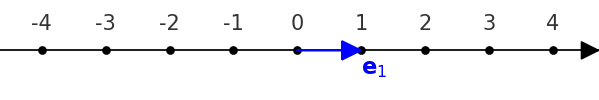
\includegraphics[width=0.4\linewidth]{Tuan2/Figures/1Dvectorspace.png}
    \end{figure}
    Rõ ràng, tập hợp các số thực \(\mathbb{R}\) cũng là một không gian vector với duy nhất một vector cơ sở là \(1\) (hoặc bất kỳ số thực nào khác). Mỗi vector có thể được biểu diễn bằng một toạ độ -một điểm trên trục số, và từ đó là toàn bộ hệ sinh.
    \item Mặt phẳng toạ độ: \(\mathbb{R}^2\)
    \begin{figure}[H]
        \centering
        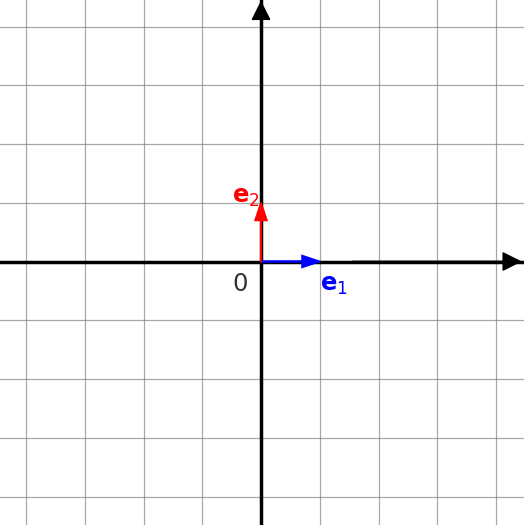
\includegraphics[width=0.4\linewidth]{Tuan2/Figures/2Dvectorspace.png}
    \end{figure}
    Với không gian vector quen thuộc này, ta kí hiệu nó là \(\mathbb{R}^2\). Hai cơ sở quen thuộc là \((1;0)\) và \((0;1)\), với mỗi vector được biểu diễn bằng hai toạ độ, và do đó là một nút của hai đường thẳng vuông góc với trục tung, trục hoành. Rồi từ đó là toàn bộ hệ sinh.
    \item Không gian hình học: \(\mathbb{R}^3\)
    \begin{figure}[H]
        \centering
        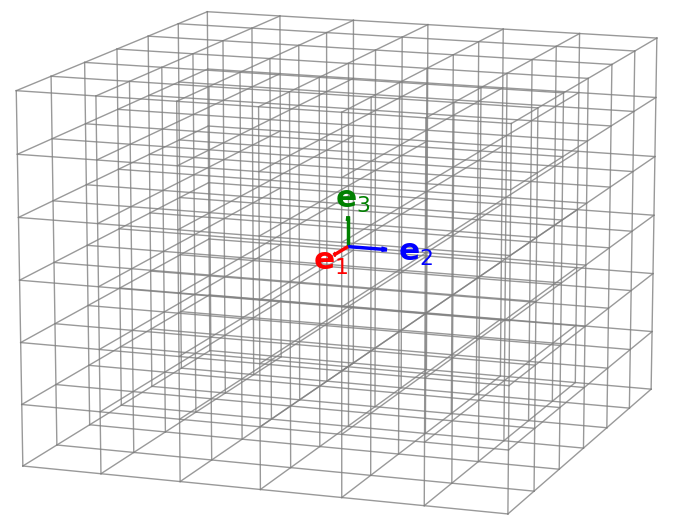
\includegraphics[width=0.4\linewidth]{Tuan2/Figures/3Dvectorspace.png}
    \end{figure}
    Với trường hợp này, ta cần ba vector cơ sở và tương ứng là ba toạ độ cho mỗi vector. Hệ sinh của không gian được minh hoạ như trong hình.
\end{enumerate}
Nhận thấy rằng các trường hợp trên khác nhau bởi số lượng của vector cơ sở\footnote{Có thể chứng minh rằng số lượng vector cơ sở cho cùng một không gian là duy nhẩt. Xem \emph{Chapter 3. Introduction to Linear Algebra. Gilbert Strange. 5th} cho một chứng minh với các vector thực.}, \textbf{khái niệm \emph{chiều} của một không gian vector vì vậy dược định nghĩa là số lượng của các vector cơ sở trong hệ cơ sở của không gian đó}. Các trường hợp có chiều là \(1,2,3\) đã được đề cập. Vậy \(4,5,\dots n\) thì sao? Ta không thể minh hoạ được các ví dụ này, nhưng có thể biểu diễn các vector trong, không gian vector \(\mathbb{R}^4\) bằng một vector có bốn toạ độ là, chẳng hạn, \((1,2,3,4)\), tức là một mảng số một chiều có bốn thành phần. Tương tự, \(n\) toạ độ cho \(\mathbb{R}^n\).
\vspace{8pt}

Ký hiệu \(\mathbb{R}^n\) chỉ rằng các vector trong không gian này có thành phần là các số thực. Điều này có thể được mở rộng sang số phức, và thậm chí còn đối với các đối tượng không phải là số. Đến lúc này, ta cần nhìn lại rằng vector là gì? Vật lý giới thiệu đến cho ta những mũi tên có thể được mô tả bởi một mảng số. Nhưng không còn mũi tên nào có thể được tưởng tượng đối với 
\(\mathbb{R}^4\) và cao hơn, thay vào đó là các mảng số. Vậy có phải vector là các mảng số nhưng được minh hoạ bằng các mũi tên? Ở phần \ref{morexample}, ta thấy rằng vector cũng có thể được hiểu là hàm số, với các thành phần là các luỹ thừa của biến. Thực ra điều này không quan trọng. 
Ta không cần phải biết vector, một cách tường minh, là cái gì hay là những cái gì. Ta chỉ đơn giản là gọi những đối tượng thuộc về cùng một tập hợp nào đó thoả mãn các tiên đề trong định nghĩa \ref{def2.2.4} là vector. Cũng dựa vào đó, các phép toán mang tính khái quát cao, gắn liền với khái niệm vector được xây dựng, áp dụng cho nhiều đối tượng; tất cả được gói gọn trong một khái niệm trừu tượng.

\subsubsection*{Không gian con}
\begin{figure}[H]
    \centering
    \begin{subfigure}[t]{0.4\textwidth}
        \centering
        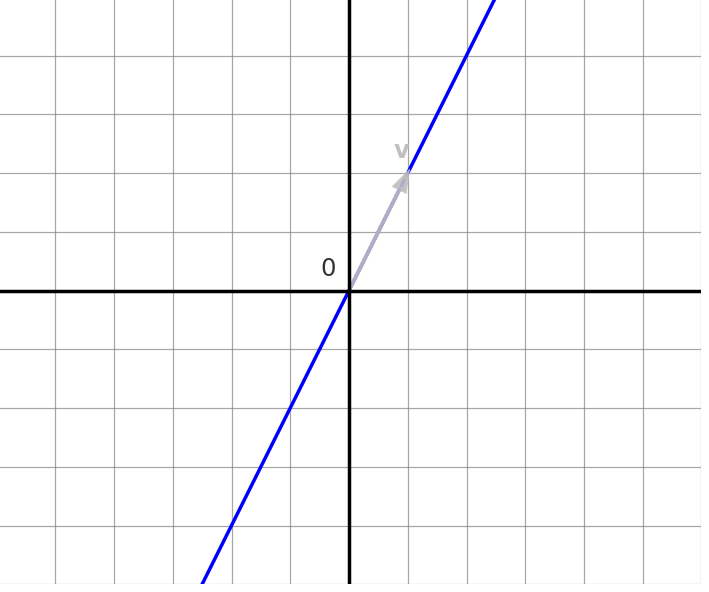
\includegraphics[width=0.8\linewidth]{Tuan2/Figures/lineonplane.png}
        \caption{Đường thẳng (đi qua gốc toạ độ) trên mặt phẳng}
    \end{subfigure}
    \hfill
    \begin{subfigure}[t]{0.4\textwidth}
        \centering
        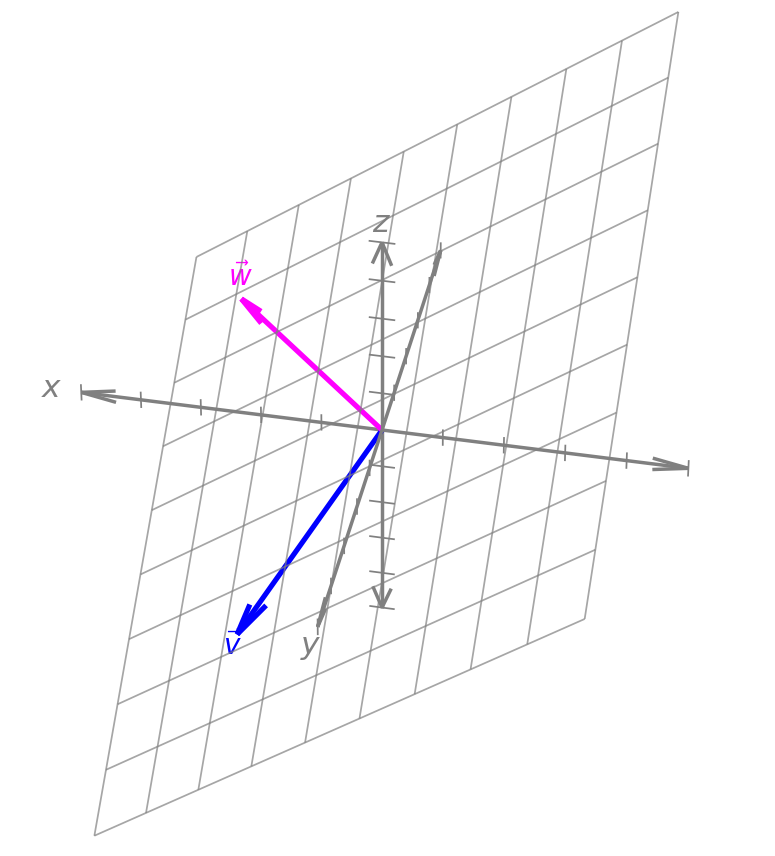
\includegraphics[width=0.8\linewidth]{Tuan2/Figures/planeinspace.png}
        \caption{Mặt phẳng (đi qua gốc toạ độ) trong không gian}
    \end{subfigure}
\end{figure}
Đây là hai ví dụ cho khái niệm \emph{không gian con}. Đầu tiên là một đường thẳng trong không gian \(\mathbb{R}^2\), 
mọi vector nằm trên đường thẳng này đều là tổ hợp tuyến tính của \(\mathbf{v}\). Tiếp theo là một mặt phẳng trong không gian \(\mathbb{R}^3\),
mọi vector trên mặt phẳng này đều là một tổ hợp tuyến tính của \(\mathbf{v}\) và \(\mathbf{w}\), hai vector độc lập tuyến tính nằm trên mặt phẳng.
Cả hai tập hợp các vector này đều thoả mãn các tiên đề trong định nghĩa \ref{def2.2.4}, nên chúng đều là các không gian vector. 

\begin{definition}
Một không gian con \(S\) trong một không gian vector \(V\) là một tập hợp các vector trong \(V\) sao cho chúng thoả mãn các tiên đề trong định nghĩa \ref{def2.2.4}.
\end{definition}

Nghĩa là mọi tổ hợp tuyến tính của các vector trong không gian con \(S\) đều nằm trong không gian con đó, và nằm trong cả \(V\).
\begin{definition}
    Một cơ sở cho một không gian con \(S\) của \(\mathbb{R}^n\) là một tập hợp các vector trong \(S\) sao cho 
    \begin{enumerate}
        \item tạo thành \(S\), và
        \item là độc lập tuyến tính.
    \end{enumerate}
\end{definition}
Hai không gian vector trong ví dụ trên đều là không gian con của \(\mathbb{R}^3\). Tương tự, nếu ta xét một đường thẳng đi qua gốc toạ độ nằm trên mặt phẳng trong ví dụ, đường thẳng này cũng là một không gian con của mặt phẳng, và đồng thời là một không gian con của \(\mathbb{R}^3\).
Hơn nữa, vector \(\mathbf{0}\) tự nó tạo thành một không gian vector, và là không gian con của chính nó cùng các không gian \(\mathbb{R}^n\) khác. Đây là lý do cần có điều kiện "đi qua gốc toạ độ".
\begin{figure}[H]
    \centering
    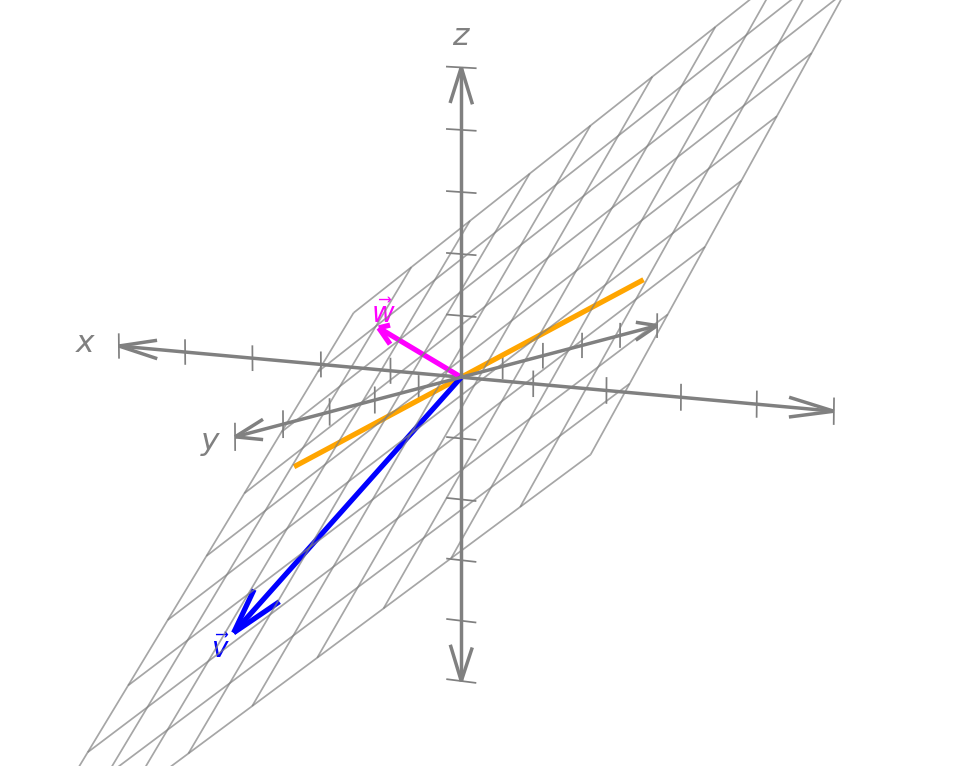
\includegraphics[width=0.6\linewidth]{Tuan2/Figures/lineonplaneinspace.png}
\end{figure}

\subsection{Giới thiệu về ma trận}
Một cái nhìn toàn cảnh về vector mang đến một trực giác về vị trí chung nhất của từng khái niệm trong bức tranh rộng lớn. Nhưng sự tương quan giữa chúng thì sao? Những liên kết, biến đổi giữa chúng thì sao? Để bắt đầu 
khảo sát, trước tiên hay làm quen với một công cụ truyền tải thông tin mạnh mẽ hơn mảng một chiều-ma trận.
\vspace{8pt}

Ta xét bảng số- mảng số hai chiều sau:
\[ \mathbf{A}=
\begin{bmatrix}
    1&5&12\\
    3&0&4\\
    0&7&9
\end{bmatrix}.
\]
Đây là một ô vuông có kích thước \(3\times 3\), tức là có \(3\) \emph{hàng} và \(3\) \emph{cột}. Hàng được đọc từ trên xuống và cột được đọc từ trái sang. Mỗi một phần tử  trong \(9\) phần tử  của bảng số này được xác định với một cặp số duy nhất của hàng và cột. Ví dụ, số \(4\) nằm ở hàng thứ hai và cột thứ ba. 
Các số \(12,4,9\) đều nằm ở cột thứ ba và các số \(3,0,4\) đều nằm ở hàng thứ hai. 

Hay ta cũng có thể lấy thêm một bảng số khác, chẳng hạn
\[\mathbf{B}=\begin{bmatrix}
    -1.3&0.6\\
    20.4&5.5\\
    9.7&-6.2
\end{bmatrix}\] Đây là một bảng số với \(3\) hàng và \(2\) cột. Nếu vẫn giữ nguyên cách đọc bảng số trước đó, thì số \(9.7\) có vị trí là hàng thứ ba, cột thứ nhất. 

Vậy ý nghĩa của những bảng số (ma trận) vừa rồi là gì? Ta hãy cùng xem xét thêm một ví dụ: hai bảng số có \(3\) hàng và \(1\) cột, 
\[\mathbf{v}=\begin{bmatrix}
    a\\b\\c
\end{bmatrix}, \quad \mathbf{w}=\begin{bmatrix}
    c\\d\\f
\end{bmatrix}.
\] Điều đáng chú ý ở đây là ta có thể gọi \(\mathbf{v}\) và \(\mathbf{w}\) là các \emph{vector}. Thật vậy, nếu ta để chúng tuân theo các quy tắc của vector, các thành phần của hai bảng số vừa rồi sẽ giống như là các thành phần của một vector. 
Nghĩa là, \[\mathbf{v}+\mathbf{w}=\begin{bmatrix}
    a+c\\b+d\\c+f
\end{bmatrix},\] hay \[
    4\cdot\mathbf{v}=\begin{bmatrix}
        4a\\4b\\4c
\end{bmatrix}.\]
Về cơ bản, đây chỉ là một sự thay đổi về cách viết. Cụ thể là thay vì viết \((a,b,c)\), ta viết \(\begin{bmatrix}
    a\\b\\c
\end{bmatrix}\). Như vậy chuyện gì xảy ra với  \(\mathbf{A}\) và \(\mathbf{B} \)? Chúng cũng là các vector (theo nghĩa trừu tượng hơn), nhưng tạm thời ta có thể chỉ cần nhìn nhận theo khía cạnh: \emph{các cột của chúng là các vector. }
\vspace{8pt}

    \emph{Ma trận là một mảng chữ nhật hoặc hình vuông (ma trận vuông) chứa các số hoặc những đối tượng toán học khác, mà có thể định nghĩa một số phép toán như cộng hoặc nhân trên các ma trận.}
\vspace{8pt}

Một ma trận \(\mathbf{A}\) có \(m\) hàng và \(n\) cột được gọi là một ma trận \(m\times n\), điều này xác dịnh độ lớn của ma trận. Ta viết \(\mathbf{A}_{m\times n}\) để chỉ ma trận \(A\) có kích thước \(m\times n\). Chú ý rằng ta đọc hàng trước cột. 
\vspace{8pt}

Về tổng quát, một ma trận \(m\times n\) có dạng
\[\begin{bmatrix}
    \mathbf{A}_{11} &   \mathbf{A}_{12} &\cdots &\mathbf{A}_{1j} &\cdots      & \mathbf{A}_{1n}\\  
    \mathbf{A}_{21} &   \mathbf{A}_{22} &\cdots &\mathbf{A}_{2j} &\cdots      & \mathbf{A}_{2n}\\
    \vdots          &   \vdots          &\ddots &\vdots          &\ddots      & \vdots         \\
    \mathbf{A}_{i1} &   \mathbf{A}_{i2} &\cdots &\mathbf{A}_{ij} &\cdots      & \mathbf{A}_{in}\\
    \vdots          &   \vdots          &\ddots &\vdots          &\ddots      &\vdots          \\
    \mathbf{A}_{m1} &   \mathbf{A}_{m2} &\cdots &\mathbf{A}_{mj} &\cdots      & \mathbf{A}_{mn}              
\end{bmatrix}.\]
\subsection{Các phép toán trên ma trận}
Cũng như với các số và vector, ta có thể thực hiện pháp cộng, trừ với các ma trận, cũng có thể nhân một số với ma trận và cuối cùng là nhân ma trận với ma trận, ma trận với vector. 
\vspace{8pt}

\textbf{Phép cộng hai ma trận.} Xét hai ma trận \(\mathbf{A}\) và \(\mathbf{B}\) có kích thước \(m\times n\), tổng của hai ma trận là một ma trận \(m\times n\) được định nghĩa là 
\begin{equation}
   \mathbf{A}_{ij}\in\mathbb{R},\quad \mathbf{B}_{ij}\in\mathbb{R},\quad 
    (\mathbf{A}+\mathbf{B})_{ij}=\mathbf{A}_{ij}+\mathbf{B}_{ij}.
\end{equation}
Chú ý rằng ta viết \(\mathbf{A}_{ij}\) để chỉ phần tử nằm ở hàng thứ \(i\) và cột thứ \(j\) của \(\mathbf{A}\), và tương tự \((\mathbf{A+B})_{ij}\) để chỉ phần tử nằm ở hàng thứ \(i\) và cột thứ \(j\) của ma trận đó. Vậy, để cộng hai ma trận, ta cộng từng phần tử lại với nhau. Điều này tương tự như phép cộng các vector.
Tương tự, chúng ta có thể nhân ma trận với một hằng số \(c\in\mathbb{R}\):
\begin{equation}
    (c\mathbf{A})_{ij}=c\mathbf{A}_{ij}.
\end{equation}
Điều này tương tự như phép nhân vô hướng với một vector. Khi \(c=-1\), ta thu được ma trận \(-\mathbf{A}\) sao cho \(\mathbf{A}+(-\mathbf{A})=\mathbf{0}\); \(\mathbf{0}\) là ma trận kích thước \(m\times n\) với mọi phần tử trong đó đều bằng \(0\).

\textbf{Ví dụ.}\[4\begin{bmatrix}
    0&3\\ 2&-6
\end{bmatrix}+\begin{bmatrix}
    1&-2\\ 0&5
\end{bmatrix}=\begin{bmatrix}
    0&12\\ 8&-24
\end{bmatrix}+\begin{bmatrix}
    1&-2\\ 0&5
\end{bmatrix}=\begin{bmatrix}
    1&10\\ 8&-19
\end{bmatrix}.\]
\vspace{8pt}

\textbf{Phép nhân ma trận-vector.} Ta hãy bắt đầu với một ví dụ. Giả sử ta có vector \[\mathbf{v}=\begin{bmatrix}
    +2\\+5\\-4
\end{bmatrix},\] vector này có thể được phân tích thành một tổ hợp tuyến tính của một hệ cơ sở nào đó, chẳng hạn
\[\begin{bmatrix}
    2\\5\\-4
\end{bmatrix}=2\begin{bmatrix}
    1\\0\\0
\end{bmatrix}+(-3)\begin{bmatrix}
    0\\2\\-5
\end{bmatrix}+1\begin{bmatrix}
    0\\11\\-19
\end{bmatrix}.\]
Bằng cách định nghĩa một phép toán mới, ta có thể viết lại thành dạng
\begin{equation}\label{eq2.2.1}
    \begin{bmatrix}
    2\\5\\-4
\end{bmatrix}=\begin{bmatrix}
    1&0&0\\
    0&2&11\\
    0&-5&-19
\end{bmatrix}\begin{bmatrix}
    2\\-3\\1
\end{bmatrix}.\end{equation} Ta đã đặt các vector cơ sở vào cột của ma trận \(3\times 3\) vừa rồi, và các hệ số của tổ hợp tuyến tính vào một vector cột. Về tổng quát, một phép nhân ma trận \(m\times n\) với một vector \(n\times 1\) sẽ cho ra một vector \(m\times 1\), và phần tử thứ \(i\) được tính bởi 
\begin{equation}
    (\mathbf{Ax})_i = \sum_{j=1}^n \mathbf{A}_{ij}\mathbf{x}_j.
\end{equation}
Cũng có thể viết thành, trong trường hợp \(n=3\),
\[\begin{bmatrix}
    \vert &\vert&\vert\\
    \mathbf{A}_{i1}&\mathbf{A}_{i2}&\mathbf{A}_{i3}\\
    \vert &\vert&\vert\\
\end{bmatrix}\begin{bmatrix}
    x_1\\x_2\\x_3
\end{bmatrix}=x_1\begin{bmatrix}
    \vert\\\mathbf{A}_{i1}\\ \vert
\end{bmatrix}+x_2 \begin{bmatrix}
    \vert\\\mathbf{A}_{i2}\\ \vert
\end{bmatrix}+x_3\begin{bmatrix}
    \vert\\\mathbf{A}_{i1}\\ \vert
\end{bmatrix}.\]
Vector mới là một tổ hợp tuyến tính của các cột của ma trận \(\mathbf{A}\) với các hệ số là các phần tử của vector \(\mathbf{x}\). Cũng dễ thấy rằng, phần tử thứ \(i\) của vector này là tích vô hướng của hàng thứ \(i\) của \(\mathbf{A}\) với vector \(\mathbf{x}\). Nghĩa là, chẳng hạn, 
\[\begin{bmatrix}
    0&2&11
\end{bmatrix}\begin{bmatrix}
    2\\-3\\1
\end{bmatrix}=\begin{bmatrix}
    0\\2\\11
\end{bmatrix}\cdot \begin{bmatrix}
    2\\-3\\1
\end{bmatrix}=0\times 2+2\times(-3)+11\times 1 =5.\]
Vì tích vô hướng có tính phân phối là \(\mathbf{a}\cdot(\mathbf{b}+\mathbf{c})=\mathbf{a}\cdot\mathbf{b}+\mathbf{a}\cdot\mathbf{c},\)
phép nhân ma trận-vector cũng có tính chất tương tự: \[\mathbf{A}(\mathbf{a}+\mathbf{b})=\mathbf{A}\mathbf{a}+\mathbf{A}\mathbf{b}.\]
\vspace{8pt}

\textbf{Phép nhân ma trận với ma trận.} Ta bắt đầu với việc biểu diễn các vector cơ sở được nhắc tới vừa rồi thông qua một hệ cơ sở khác.
\begin{align*}&\begin{bmatrix}
    1\\0\\0
\end{bmatrix}=1\begin{bmatrix}
    0.5 \\-1\\0
\end{bmatrix}+2\begin{bmatrix}
    0.75 \\1\\-2
\end{bmatrix}+1\begin{bmatrix}
    -1 \\-1\\4
\end{bmatrix},\\
&\begin{bmatrix}
    0\\2\\-5
\end{bmatrix}=-1.625\begin{bmatrix}
    0.5\\-1\\0
\end{bmatrix}-1.75\begin{bmatrix}
    0.75\\-1\\0
\end{bmatrix}-2.125\begin{bmatrix}
    -1\\-1\\4
\end{bmatrix},\\
&\begin{bmatrix}
    0\\11\\-19
\end{bmatrix}=-7.875\begin{bmatrix}
    0.5\\-1\\0
\end{bmatrix}-3.25\begin{bmatrix}
    0.75\\-1\\0
\end{bmatrix}-6.375\begin{bmatrix}
    -1\\-1\\4
\end{bmatrix}.
\end{align*}
Các tổng này, như đã biết, có thể được viết thành tích của một ma trận và một vector:
\begin{align*}
    &\begin{bmatrix}
        1\\0\\0
    \end{bmatrix}=\begin{bmatrix}
        0.5 & 0.75 & -1\\
        -1 & 1 & -1\\
        0 & -2 & 4
    \end{bmatrix}\begin{bmatrix} 1\\2\\1\end{bmatrix},\\
&\begin{bmatrix}
    0\\2\\-5
\end{bmatrix}=\begin{bmatrix}
    0.5 & 0.75 & -1\\
    -1 & 1 & -1\\
    0 & -2 & 4
\end{bmatrix}\begin{bmatrix}
    -1.625\\-1.75\\-2.125
\end{bmatrix}\\
&\begin{bmatrix}
    0\\11\\-19
\end{bmatrix}=\begin{bmatrix}
    0.5 & 0.75 & -1\\
    -1 & 1 & -1\\
    0 & -2 & 4
\end{bmatrix}\begin{bmatrix}
    -7.875\\-3.25\\-6.375
\end{bmatrix}.
\end{align*} Gọi ma trận \(3\times 3\) ở vế phải là \(\mathbf{B}\), thay vào \eqref{eq2.2.1},
\[\begin{bmatrix}
    2\\5\\-4
\end{bmatrix}=\begin{bmatrix}
    \mathbf{B}\begin{bmatrix}
        1\\2\\1
    \end{bmatrix}&\mathbf{B}\begin{bmatrix}
        -1.625\\-1.75\\-2.125
    \end{bmatrix}&\mathbf{B}\begin{bmatrix}
        -7.875\\-3.25\\-6.375
\end{bmatrix}\end{bmatrix}\begin{bmatrix}
2\\-3\\1
\end{bmatrix}.\] Quan sát phương trình này, ta nhận thấy sự lặp của \(\mathbf{B}\); điều này liên tưởng ta đến một phép nhân. 
Tức là, ta có thể viết 
\begin{equation}\label{eqmatrix}\begin{bmatrix}
    2\\5\\-4
\end{bmatrix}=\mathbf{B}\begin{bmatrix}
    1&-1.625&-7.875\\
    2&-1.75&-3.25\\
    1&-2.125&-6.375
\end{bmatrix}\begin{bmatrix}
    2\\-3\\1
\end{bmatrix},\end{equation} bằng cách định nghĩa một phép nhân mới, và ta gọi phép nhân này là một phép nhân ma trận với ma trận.
\vspace{8pt}

Xét một ma trận \(\mathbf{A}_{m\times n}\) và một ma trận \(\mathbf{B}_{n\times p}\), \emph{tích của của chúng là một ma trận \(\mathbf{C}_{m\times p}\); các cột của ma trận này là các vector, bằng với tích ma trận-vector của ma trận \(\mathbf{A}\) và các cột tương ứng  của ma trận \(B\).}
\vspace{8pt}

Đồng thời, ta cũng nhận thấy rằng tích ma trận-vector cũng là một tích ma trận-ma trận, vì vector là một ma trận có một cột. Do đó, để tổng quát, ta định nghĩa phép nhân ma trận với ma trận như sau: 
\begin{equation}\label{eq2.2.2}
    \mathbf{C}_{ij}=(\mathbf{AB})_{ij}=\sum_{k=1}^n \mathbf{A}_{ik}\mathbf{B}_{kj}.
\end{equation}
Hay, nói cách khác, phần tử thứ \((i,j)\) của \(\mathbf{C}\) bằng tích vô hướng của hàng thứ \(i\) của ma trận \(\mathbf{A}\) với cột thứ \(j\) của ma trận \(\mathbf{B}\).
\begin{figure}[H]
    \centering
    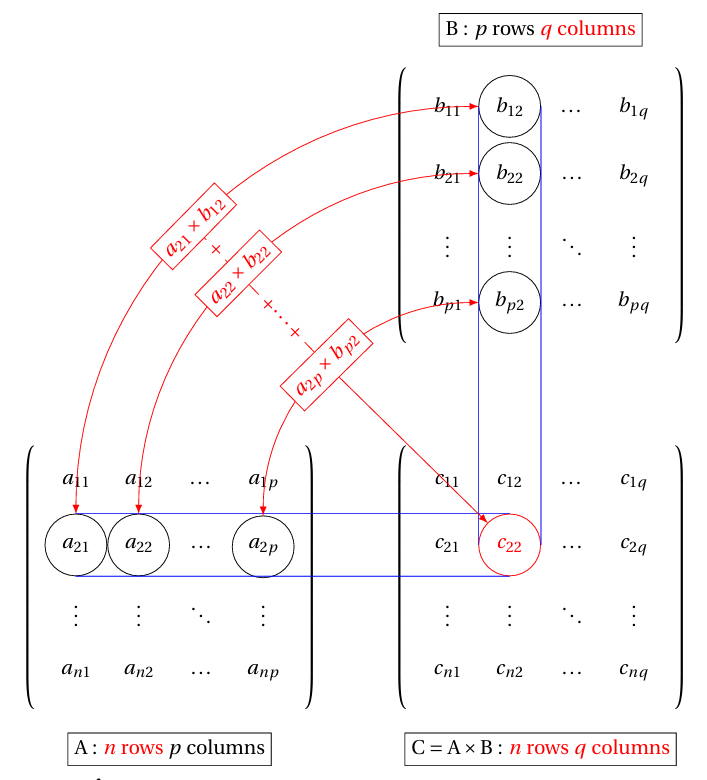
\includegraphics[width=0.5\linewidth]{Tuan2/Figures/matricemultiplication.png}
\end{figure}
Một đẳng thức vector mà ta thường gặp tương đương với ba (hoặc hai) đẳng thức đại số. Còn, như ta đã thấy, hệ hai đẳng thức \eqref{eqmatrix} và \eqref{eq2.2.1} tương đương với bốn đẳng thức vector, tức là tận 12 đẳng thức đại số. Điều này chứng tỏ khả năng nén thông tin của ma trận. Một lượng rất lớn thông tin có thể được nén lại trong một ma trận, và ta có thể thực hiện các phép toán trên đó để đồng thời xử lý chúng. 
\vspace{8pt}

Để kết thúc phần này, ta hãy xét thêm một ví dụ. Hãy tính tích
\[\begin{bmatrix}
    1&5\\ 3&2
\end{bmatrix}\begin{bmatrix}
    2&-1\\ 0&3
\end{bmatrix}\] theo hai cách: \eqref{eq2.2.2} và bằng góc nhìn của phép nhân vector.

\emph{Giải.} Theo \eqref{eq2.2.2}, tích này bằng 
\[\begin{bmatrix}
    (1\cdot 2+5\cdot 0)&(1\cdot -1+5\cdot 3)\\
   ( 3\cdot 2+2\cdot 0)&(3\cdot -1+2\cdot 3)
\end{bmatrix}=\begin{bmatrix}
    2&14\\
    6&3
\end{bmatrix}.\]
Theo góc nhìn của phép nhân vector, tích này tương đương với 
\[\begin{bmatrix}
    \begin{bmatrix}
        1&5\\3&2
    \end{bmatrix}\begin{bmatrix}
        2\\0
    \end{bmatrix} &\begin{bmatrix}
        1&5\\3&2
    \end{bmatrix}\begin{bmatrix}
        -1\\3
    \end{bmatrix}
\end{bmatrix}.\]
Dễ thấy, \begin{align*}
    &\begin{bmatrix}
        1&5\\3&2
    \end{bmatrix}\begin{bmatrix}
        2\\0
    \end{bmatrix}=2\begin{bmatrix}
        1\\3
    \end{bmatrix}+0\begin{bmatrix}
        5\\2
    \end{bmatrix}=\begin{bmatrix}
        2\\6
    \end{bmatrix},\\
    &\begin{bmatrix}
        1&5\\3&2
    \end{bmatrix}\begin{bmatrix}
        -1\\3
    \end{bmatrix}=-1\begin{bmatrix}
        1\\3
    \end{bmatrix}+3\begin{bmatrix}
        5\\2
    \end{bmatrix}=\begin{bmatrix}
        14\\3
    \end{bmatrix}.
\end{align*}
\vspace{8pt}

\textbf{Các quy tắc cho các phép toán trên ma trận.} Ta tổng kết lại các quy tắc chung nhất.
Tiếp tục xét các ma trận \(\mathbf{A},\mathbf{B}\), và \(\mathbf{C}\) có kích thước phù hợp-hai ma trận để cộng được với nhau cần có cùng kích thước, để nhân được với nhau cần có số cột của ma trận bên trái bằng với số hàng của ma trận bên phải:
\begin{enumerate}[label=(\alph*)]
    \item Quy luật giao hoán: \(\mathbf{A}+\mathbf{B}=\mathbf{B}+\mathbf{A}.\)
    \item Quy luật phân phối: \(\alpha(\mathbf{A}+\mathbf{B})=\alpha\mathbf{A}+\alpha\mathbf{B}.\)
    \item Quy luật liên kết: \(\mathbf{A}+(\mathbf{B}+\mathbf{C})=(\mathbf{A}+\mathbf{B})+\mathbf{C}.\)
    \item Quy luật liên kết: \((\mathbf{AB})\mathbf{C}=\mathbf{A}(\mathbf{BC}).\)
    \item Quy luật phân phối (trái): \(\mathbf{A}(\mathbf{B}+\mathbf{C})=\mathbf{AB}+\mathbf{AC}.\)
    \item Quy luật phân phối (phải): \((\mathbf{A}+\mathbf{B})\mathbf{C}=\mathbf{AC}+\mathbf{BC}.\)
    \item Quy luật giao hoán: \(\mathbf{AB} \neq \mathbf{BA}\).
\end{enumerate}
Chú ý quy luật cuối cùng, tích ma trận không mang tính giao hoán.
\vspace{8pt}

\textbf{Ma trận chuyển vị.}
\begin{definition}
    Ma trận chuyển vị của ma trận \(\mathbf{A}\), ký hiệu là \(\mathbf{A}^T\), là ma trận có các thành phần sao cho \[(\mathbf{A}^T)_{ij}=\mathbf{A}_{ji}.\]
\end{definition}
Ví dụ: \[\mathbf{A}=\begin{bmatrix}
    1&2\\3&4
\end{bmatrix}\implies \mathbf{A}^T =\begin{bmatrix}
    1&3\\2&4
\end{bmatrix}.\] Ta thấy các thành phần nằm trên đường chéo của ma trận sẽ vẫn giữ nguyên vị trí sau chuyển vị.
Phép chuyển vị có một tính chất quan trọng là đổi thứ tự của phép nhân ma trận, cụ thể 
\[(\mathbf{AB})^T =\mathbf{B}^T \mathbf{A}^T .\] Đồng thời, đối với một các vector được biểu diễn trong (và chỉ trong) một hệ cơ sở trực chuẩn, tích vô hướng giữa hai vector chính là phép nhân ma trận 
giữa một trong hai vector đó với chuyển vị của vector còn lại. Thật vậy, 
\[\mathbf{v}\cdot \mathbf{u}=\mathbf{v}^T \mathbf{u}=\mathbf{u}^T \mathbf{v}.\] 
Ví dụ: \[\begin{bmatrix}
    1\\2
\end{bmatrix}\cdot\begin{bmatrix}
    -1\\3
\end{bmatrix}=\begin{bmatrix}
    1&2
\end{bmatrix}\begin{bmatrix}
    -1\\3
\end{bmatrix}=5.\]
\subsection{Phép biến đổi tuyến tính}
Vector, và rồi ma trận đã được giới thiệu cùng cách chúng vận hành. Vậy liệu có một ý nghĩa cốt lõi nào đó nằm đằng sau tất cả những biểu thức toán đó?  
\subsubsection*{Hệ phương trình tuyến tính}
Đây là một hệ hai phương trình tuyến tính ở dạng tổng quát:
\begin{align*}
a_{11}x_{1} + a_{12}x_{2} &= b_{1}, \\
a_{21}x_{1} + a_{22}x_{2} &= b_{2}.
\end{align*}
Một cách viết tương đương tận dụng vector là
\[\begin{bmatrix}
    a_{11}\\a_{21}
\end{bmatrix}x_{1}+\begin{bmatrix}
    a_{12}\\a_{22}
\end{bmatrix}x_{2}=\begin{bmatrix}
    b_{1}\\b_{2}
\end{bmatrix},\] hay,
\[\begin{bmatrix}
    a_{11}&a_{12}\\
    a_{21}&a_{22}
\end{bmatrix}\begin{bmatrix}
    x_{1}\\x_{2}
\end{bmatrix}=\begin{bmatrix}
    b_{1}\\b_{2}
\end{bmatrix}.\] Phương trình này có thể được viết lại thành thành \[\mathbf{A}\mathbf{x}=\mathbf{b}.\]
Đồng thời, sau khi giải hệ phương trình kia, nghiệm thu được sẽ có dạng
\begin{align*}
x_{1} &= a_{11}^{-1}b_{1} + a_{12}^{-1}b_{2}, \\
x_{2} &= a_{21}^{-1}b_{1} + a_{22}^{-1}b_{2}.
\end{align*}
Với \(a_{ij}^{-1}\) là một con số nào đó có vị trí tương ứng với \(a_{ij}\); và hệ này cũng tương đương Với
\[\begin{bmatrix}
    x_{1}\\x_{2}
\end{bmatrix}=\begin{bmatrix}
    a_{11}^{-1}&a_{12}^{-1}\\
    a_{21}^{-1}&a_{22}^{-1}
\end{bmatrix}\begin{bmatrix}
    b_{1}\\b_{2}
\end{bmatrix}.\] Nói cách khác, \[\mathbf{x}=\mathbf{A}^{-1}\mathbf{b}.\]
Ta gọi \(\mathbf{A^{-1}}\) là ma trận nghịch đảo của \(\mathbf{A}\). Dễ thấy, nghịch đảo của nghịch đảo của một ma trận là chính nó, điều này nghĩa là
\[\mathbf{A}\mathbf{A}^{-1}=\mathbf{A}^{-1}\mathbf{A}=\mathbf{I}.\] Ma trận \(\mathbf{I}\) được gọi là ma trận đơn vị, tất cả phần tử trong ma trận vuông này đều bằng 0, trừ các phần tử nằm trên đường chéo, bằng nhau và bằng 1. Đặc tính của nó là 
\[\mathbf{I}\mathbf{x}=\mathbf{x}.\] Một số ví dụ cho \(\mathbf{I}\):
\[\begin{bmatrix}
    1&0\\
    0&1
\end{bmatrix},\quad
\begin{bmatrix}
    1&0&0\\
    0&1&0\\
    0&0&1
\end{bmatrix}.\]
Ngoài ra, có thể dễ dàng chứng minh rằng 
\[\mathbf{C}=\mathbf{AB}\implies \mathbf{C}^{-1}=\mathbf{B}^{-1}\mathbf{A}^{-1}.\] Đây sẽ là một bài tập nhỏ.
\subsubsection*{Toán tử tuyến tính}
Từ những gì mới biết được, hãy làm một so sánh nhỏ:
\begin{center}
\begin{tabular}{|c|c|c|}
  \hline
   & Ma trận & Hàm số \\
  \hline
  Dạng chuẩn & \(\mathbf{A}\mathbf{x}=\mathbf{b}\) & \(f(x)=y\) \\
  \hline
   Nghịch đảo& \(\mathbf{x}=\mathbf{A}^{-1}\mathbf{b}\) & \(x=f^{-1}(y)\) \\
  \hline
\end{tabular}
\end{center}
Như vậy thì việc nhân một ma trận với một vector là tương đồng với đặt vector đó làm đầu vào của một hàm, và đầu ra của một hàm như vậy là một vector khác.
Tuy nhiên, thay vì dùng từ \emph{hàm}, một thuật ngữ mới được sử dụng: \emph{biến đổi}. Đối với một vector \(\mathbf{u}\in\mathbb{R}^n\), một biến đổi \(T\)\footnote{T: transformation=map} biến
nó thành một vector mới \(\mathbf{v}\in\mathbb{R}^m\). Ngược lại, một biến đổi \(T^{-1}\) sẽ trả \(\mathbf{v}\) trở lại \(\mathbf{u}\). Nhưng có phải ta luôn có 
\[\mathbf{A}\mathbf{x}=T(\mathbf{x})\] không? Không. Giả sử xét một biến đổi 
\[T\left(\begin{bmatrix}
    x_1\\x_2
\end{bmatrix}\right)=\begin{bmatrix}
    x_{1}^2 +x_{2}^2 \\x_{1}^2 -x_{2}^2
\end{bmatrix},\] ta sẽ không thể tìm thấy một ma trận nào làm được điều này cả. Và hoá ra là bảng so sánh của ta thiếu một số thứ quan trọng:
\begin{center}
\begin{tabular}{|c|c|c|}
  \hline
   & Ma trận & Hàm số \\
  \hline
  Dạng chuẩn & \(\mathbf{A}\mathbf{x}=\mathbf{b}\) & \(f(x)=y\) \\
  \hline
   Nghịch đảo& \(\mathbf{x}=\mathbf{A}^{-1}\mathbf{b}\) & \(x=f^{-1}(y)\) \\
  \hline
  Tính tuyến tính & \(\mathbf{A}(\mathbf{x}_1+\mathbf{x}_2)=\mathbf{A}\mathbf{x}_1 +\mathbf{A}\mathbf{x}_2\) &\(f(x_1 +x_2)=f(x_1)+f(x_2)\)\\
  Tính đồng nhất & \(\mathbf{A}(\alpha\mathbf{x})=\alpha\mathbf{A}\mathbf{x}\)&\(f(\alpha x)=\alpha f(x)\)\\
  \hline
\end{tabular}
\end{center}
Một hàm số có đầy đủ tính chất như trong bảng đề cập được gọi là một hàm tuyến tính; do đó, phép biến đổi mà ta cần quan tâm đến cũng phải là một biến đổi tuyến tính. Vì vậy, ma trận được gọi là một \textbf{\emph{toán tử tuyến tính}}.
\begin{definition}
    Một biến đổi tuyến tính\footnote{L: linear transformation} là biến đổi \(L: \mathbb{R}^n \rightarrow\mathbb{R}^m\) thoả mãn hai đặc tính:
    \[\text{tuyến tính:}\quad L(\mathbf{u}+\mathbf{v})=L(\mathbf{u})+L(\mathbf{v}),\]
    \[\text{tuyến tính:}\quad L(\alpha\mathbf{v})=\alpha L(\mathbf{v}).\]
\end{definition}
Từ đây dễ dàng chứng minh được hai hệ quả quan trọng:
\begin{enumerate}
    \item \(L(\mathbf{0})=\mathbf{0}\).
    \item \(L(\alpha_{1}\mathbf{e}_1+\alpha_2 \mathbf{e}_2 +\cdots +\alpha_n \mathbf{e}_{n})=\alpha_1 L(\mathbf{e}_1)+\alpha_2 L(\mathbf{e}_2)+\cdots +\alpha_n L(\mathbf{e}_n)\).
\end{enumerate}
Hệ quả 2 nói rằng nếu \(\mathbf{x}\) là một tổ hợp tuyến tính của một tập hợp các vector, \(L(\mathbf{x})\) vẫn là chính tổ hợp tuyến tính đó của tập hợp chính các vector đó sau biến đổi. 
Đồng thời có thể viết lại hệ quả 2 theo ngôn ngữ ma trận:
\[L(\mathbf{x})=\begin{bmatrix}
    \lvert & \lvert &\lvert &\lvert\\
    L(\mathbf{e}_1)&L(\mathbf{e}_2)&\cdots&L(\mathbf{e}_n)\\
     \lvert & \lvert &\lvert &\lvert
\end{bmatrix}\begin{bmatrix}
    \alpha_1 \\\alpha_2 \\\vdots\\ \alpha_n
\end{bmatrix},\] hay \[L(\mathbf{x})=\mathbf{A}\mathbf{x}.\]
\(\mathbf{A}\) được gọi là ma trận chuẩn của biến đổi \(L\). Hãy lấy ví dụ đơn giản cho một biến đổi kéo với 
\[L\left(\begin{bmatrix}
    x_1 \\x_2
\end{bmatrix}\right)=\begin{bmatrix}
    x_1 +2x_2 \\x_2
\end{bmatrix}.\] Áp dụng biến đổi này lên hai vector đơn vị \(\mathbf{e}_1 =(1,0)\) và \(\mathbf{e}_2 =(0,1)\):
\[\mathbf{e}_1 \rightarrow (1,0),\qquad \mathbf{e}_2 \rightarrow (2,1).\] Với một vector \(\mathbf{x}=(1,1)\):
\[\mathbf{x}=\begin{bmatrix}
1\\1
\end{bmatrix}\rightarrow 1\begin{bmatrix}
1\\0
\end{bmatrix}+1\begin{bmatrix}
2\\1
\end{bmatrix}=\begin{bmatrix}
    1&2\\0&1
\end{bmatrix}\begin{bmatrix}
    1\\1
\end{bmatrix}=\begin{bmatrix}
    3\\1
\end{bmatrix}.\]
\subsubsection*{Sự kết hợp các biến đổi tuyến tính}
Một sự gợi nhắc về hàm hợp cho ta liên tưởng đến trường hợp tương tự cho phép biến đổi hợp. Nói cách khác, một phép biến đổi hợp là một phép biến đổi lấy đều vào là đầu ra của một phép biến đổi khác:
\[L_2 (L_1 (\mathbf{v}))=L(\mathbf{v})=\mathbf{w}.\] Trong ngữ cảnh của toán tử tuyến tính tương ứng với phép biến đổi tuyến tính, điều này chính là một phép nhân ma trận của các ma trận chuẩn
\[\mathbf{B}(\mathbf{A}\mathbf{x})=(\mathbf{BA})\mathbf{x}.\]
Với sự chồng chập của liên tiếp 3 biến đổi tuyến tính,
\[L_3 (L_2 (L_1 (\mathbf{v})))=L(\mathbf{v})=\mathbf{C}(\mathbf{B}(\mathbf{A}\mathbf{x})).\] Từ đây ta dễ dàng chứng minh quy luật liên kết
\[\mathbf{C}(\mathbf{BA})=(\mathbf{CB})\mathbf{A}=(\mathbf{C}\mathbf{B}\mathbf{A}).\]
\subsubsection*{Minh hoạ cho phép biến đổi tuyến tính}
Có thể thấy rằng một phép biến đổi \(L: \mathbb{R}^n \rightarrow \mathbb{R}^m\) có toán tử tuyến tính tương ứng là một ma trận \(m\times n\); nhưng
sau đây ta sẽ chủ yếu minh hoạ cho trường hợp \(m=n\), tức ma trận chuẩn là một ma trận vuông \(n\times n\), do đó phép biến đổi giữ nguyên chiều của không gian vector.

\begin{figure}[H]
    \centering
    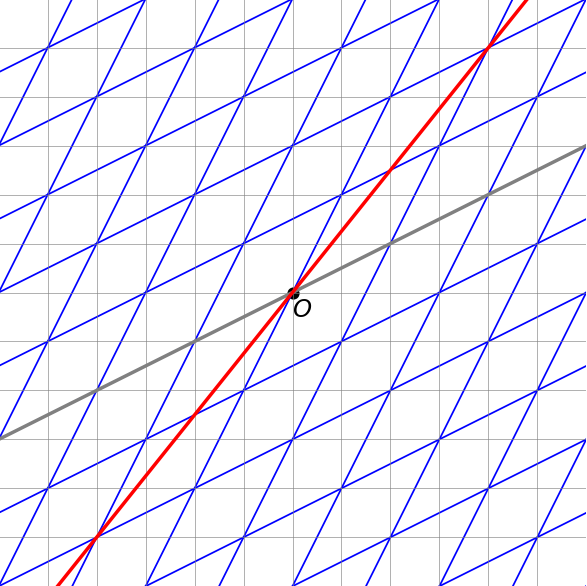
\includegraphics[width=0.5\linewidth]{Tuan2/Figures/LT1.png}
    \caption{Một phép biến đổi tuyến tính}
    \label{LT1}
\end{figure}
Hình \ref{LT1} là một minh hoạ cho phép biến đổi tuyến tính ứng với ma trận \[\mathbf{A}=\begin{bmatrix}
    1&2\\2&1
\end{bmatrix},\] các nút của lưới màu xanh thể hiện cho các vector sau biến đổi, điểm O vẫn ở nguyên chỗ (hệ quả 1), đường thẳng màu đỏ là đường thẳng màu xám sau biến đổi.
Ta tổng kết các tiêu chí cho hình ảnh của "lưới" sau một phép biến đổi tuyến tính\footnote{Xem trong 3Blue1Brown cho các hình ảnh về phép biến đổi phi tuyến}:
\begin{itemize}
    \item Điểm O giữa nguyên vị trí.
    \item Các đường kẻ của lưới song song và cách đều nhau.
    \item Một đường thẳng vẫn là một đường thẳng.
\end{itemize}
\begin{figure}[H]
    \centering
    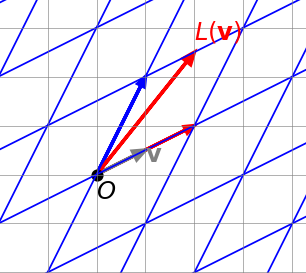
\includegraphics[width=0.4\linewidth]{Tuan2/Figures/LT2.png}
    \caption{}
    \label{LT2}
\end{figure}
Vẫn xét biến đổi đó, hình \ref{LT2} thể hiện sự biến đổi của vector \(\mathbf{v}\):
\[\mathbf{v}=\begin{bmatrix}
    1\\0.5
\end{bmatrix}\rightarrow L\rightarrow L(\mathbf{v})=\begin{bmatrix}
    2\\2.5
\end{bmatrix}.\] Nhắc lại, ta đạt được  điều này bằng cách nhân \(\mathbf{v}\) với ma trận chuẩn \(\mathbf{A}\), đây đơn giản là lấy 1 nhân với \(L(\mathbf{e}_1)\) (cột thứ nhất của \(\mathbf{A}\)) rồi cộng với 0.5 nhân \(L(\mathbf{e}_2)\) (cột thứ hai của \(\mathbf{A}\)).
Để biến đổi ngược từ "lưới" hiện tại về "lưới" vuông đằng sau, ta chỉ cần áp dụng một biến đổi với ma trận \(\mathbf{A}^{-1}\) là ma trận nghịch đảo của \(\mathbf{A}\).
\vspace{8pt}

Vậy là ta đã có một hình ảnh trực quan về phép biến đổi tuyến tính. Tiếp đến sẽ là một số phép biến đổi điển hình.
\vspace{8pt}

\emph{Phép biến đổi cắt.}\newline
Phương trình cho một biến đổi cắt 2D là 
\[
L\left(\begin{bmatrix}
    x_1 \\x_2
 \end{bmatrix}\right)=\begin{bmatrix}
    x_1 +\lambda x_2 \\x_2
 \end{bmatrix}, \text{ hoặc}\quad 
 \begin{bmatrix}
    x_1 \\\lambda x_1 +x_2
 \end{bmatrix}.
\] Tương ứng, ma trận đặc trưng là 
\[\begin{bmatrix}
    1&\lambda\\0&1
\end{bmatrix},\] hoặc 
\[\begin{bmatrix}
    1&0\\\lambda&1
\end{bmatrix}.\]
Rõ ràng ở trên ta đã có một ví dụ với ma trận 
\[
\begin{bmatrix}
    1&2\\0&1
 \end{bmatrix},
\]
 dễ thấy rằng cơ sở thứ nhất được giữ nguyên, chỉ có cơ sở thứ hai được kéo chéo sang phải; và minh hoạ cho nó là 
 \begin{figure}[H]
    \centering
    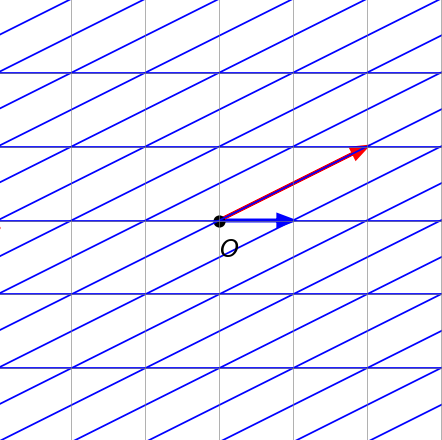
\includegraphics[width=0.4\linewidth]{Tuan2/Figures/LT3}
 \end{figure}
Nếu hình ảnh này trông quen thuộc, bạn có thể đã đoán được phần nào: phép biến đổi được thể hiện trong Hình~\ref{LT1} chính là kết hợp của hai phép biến đổi cắt và gần giống cắt.
Thực vậy,
\[
\begin{bmatrix}
    1&2\\2&1
 \end{bmatrix}=
 \begin{bmatrix}
    1&0\\2&1
 \end{bmatrix}
 \begin{bmatrix}
    1&2\\0&-3
 \end{bmatrix}.
\]
Nghĩa là ta trước tiên áp dụng ma trận biến đổi 
\[
\mathbf{A}_1 =
\begin{bmatrix}
    1&2\\0&-3
 \end{bmatrix},
\]
rồi lại biến đổi thông qua ma trận 
\[
\mathbf{A}_2 =
\begin{bmatrix}
    1&0\\2&1
 \end{bmatrix}.
\]
 \begin{figure}[H]
    \centering
    \begin{subfigure}[t]{0.48\textwidth}
        \centering
        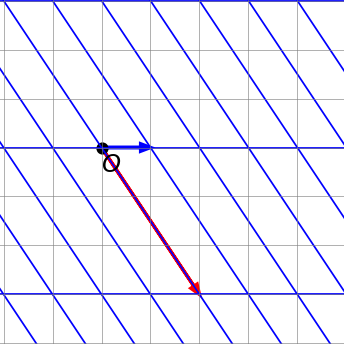
\includegraphics[width=0.9\linewidth]{Tuan2/Figures/LT4.png}
        \caption{Phép biến đổi của \(\mathbf{A}_1\)}
    \end{subfigure}
    \hfill
    \begin{subfigure}[t]{0.48\textwidth}
        \centering
        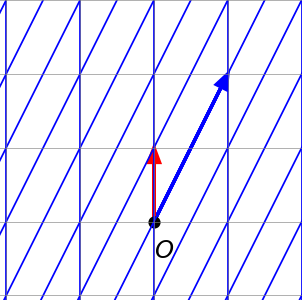
\includegraphics[width=0.9\linewidth]{Tuan2/Figures/LT5.png}
        \caption{Phép biến đổi của \(\mathbf{A}_2\)}
    \end{subfigure}
 \end{figure}
 Ta có thể đọc thấu đáo sự kết hợp này: \(\mathbf{A}_1\) chỉ thay đổi \(\mathbf{e}_2\) về cột thứ hai của \(\mathbf{A}_2\), rồi tiếp đó \(\mathbf{A}_2\) chỉ thay đổi \(\mathbf{e}_1\) về cột thứ nhất của \(\mathbf{A}\).
 \vspace{8pt}

\emph{Phép giãn nở.}\newline
Biến đổi cho một giãn nở 2D là 
\[L\left(\begin{bmatrix}
    x_1 \\x_2
\end{bmatrix}\right)=\begin{bmatrix}
    \lambda_1 x_1 \\\lambda_2 x_2
\end{bmatrix}.\] Như vậy ma trận chuẩn cho phép biến đổi này là một ma trận đường chéo,  có dạng
\[\mathbf{D}=\begin{bmatrix}
    \lambda_1 &0\\0&\lambda_2
\end{bmatrix}.\] Sau đây là ví dụ cho \(\lambda_1=3, \lambda_2 =5\):
\begin{figure}[H]
    \centering
    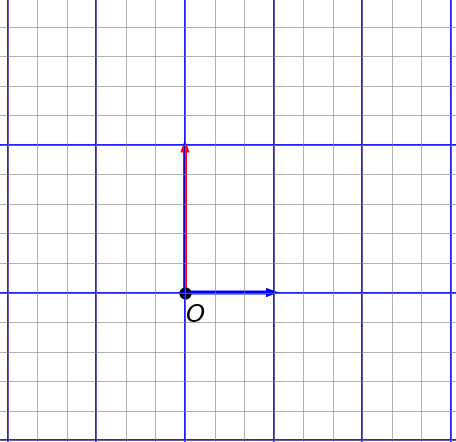
\includegraphics[width=0.5\linewidth]{Tuan2/Figures/LT6}
\end{figure}
Chú ý rằng, 
\[\mathbf{D}^{-1}=\begin{bmatrix}
    \lambda_{1}^{-1}&0\\0&\lambda_{2}^{-1}
\end{bmatrix}.\]
\emph{Phép quay.}\newline Đây là một biến đổi đặc biệt. Các vector sau biến đổi giữ nguyên độ lớn, nhưng đầu mút được quay đi một góc \(\theta\) bất kỳ nào đó.
\begin{figure}[H]
    \centering
    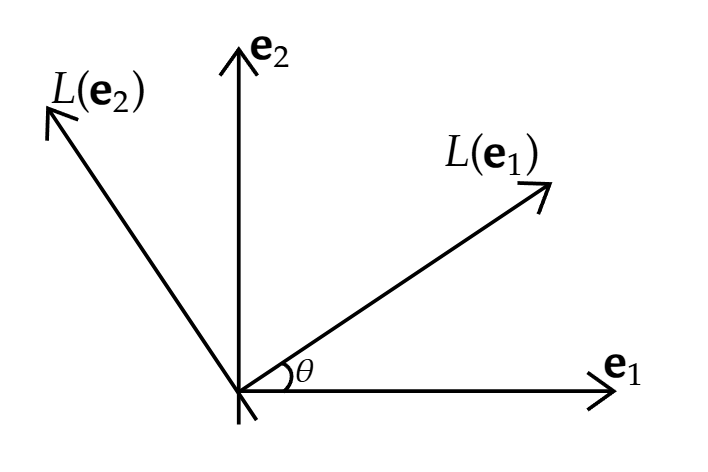
\includegraphics[width=0.6\linewidth]{Tuan2/Figures/rotation.png}
\end{figure}
Ma trận chuẩn cho phép quay 2D là 
\[\mathbf{R}=\begin{bmatrix}
    \cos\theta &-\sin\theta\\
    \sin\theta &\cos\theta
\end{bmatrix}.\] Đối với các cơ sở trực chuẩn, có một tính chất đặc biệt cần lưu ý là 
\[\mathbf{R}^{-1}=\mathbf{R}^T .\] Một số ví dụ cụ thể:
\begin{enumerate}
    \item Phép quay 90 độ theo chiều dương \[\mathbf{R}=\begin{bmatrix}
        0&-1\\1&0
    \end{bmatrix}.\]
    \begin{figure}[H]
        \centering
        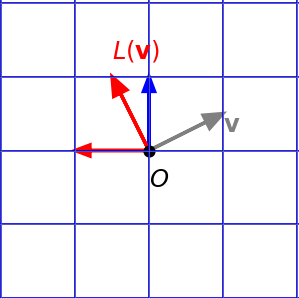
\includegraphics[width=0.3\linewidth]{Tuan2/Figures/LT7.png}
    \end{figure}
    \item Phép quay 90 độ theo chiều âm: \[\mathbf{R}=\begin{bmatrix}
        0&1\\-1&0
    \end{bmatrix}.\]
    \item Phép quay 30 độ theo chiều dương: \begin{figure}[H]
        \centering
        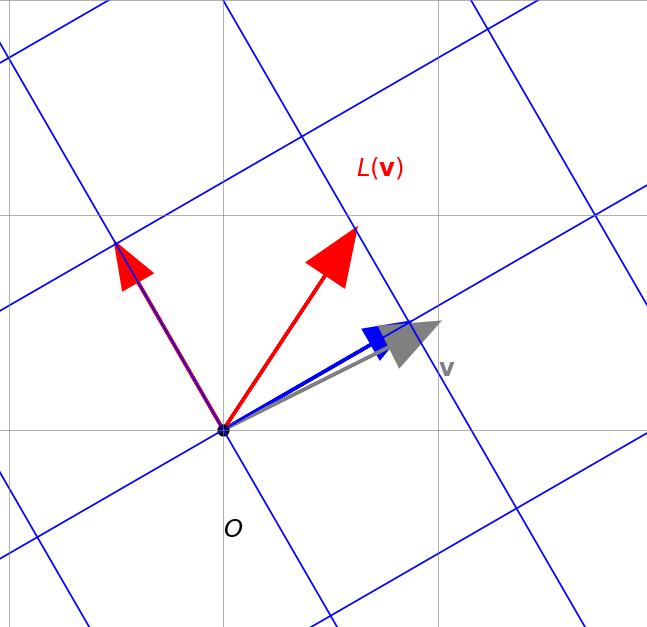
\includegraphics[width=0.3\linewidth]{Tuan2/Figures/LT8.png}
    \end{figure}
    \item Kéo rồi quay 90 độ:
    \[\begin{bmatrix}
        0&-1\\1&0
    \end{bmatrix}\begin{bmatrix}
        1&1\\0&1
    \end{bmatrix}.\] \begin{figure}[H]
        \centering
        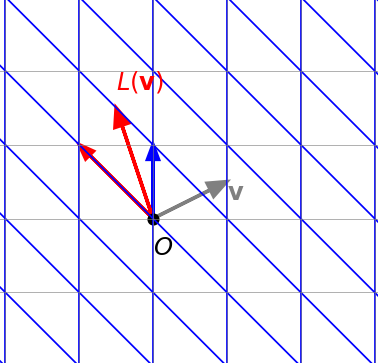
\includegraphics[width=0.3\linewidth]{Tuan2/Figures/LT9.png}
    \end{figure}
\end{enumerate}
Hãy xem 3Blue1Brown cho một trực quan hoá biến đổi tuyến tính 3D.
\subsubsection*{Định thức}
Một điều hữu dụng bất ngờ khi nghiên cứu một phép biến đổi là đánh giá rằng một phép biến đổi như thế đã kéo giãn hay ép nhỏ một thứ đi bao nhiêu;
cụ thể với trường hợp 2D, đó là nghiên cứu tỷ lệ đặc trưng của sự tăng hay giảm của diện tích một vùng trên mặt phẳng. 
\begin{figure}[H]
    \centering
    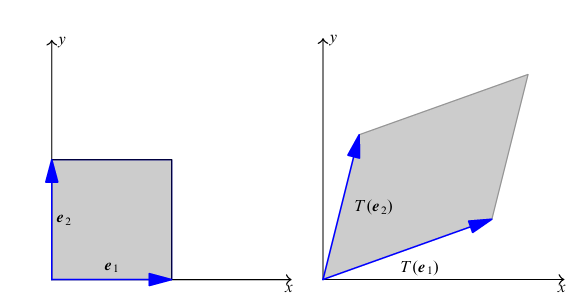
\includegraphics[width=0.6\linewidth]{Tuan2/Figures/det1.png}\
    \caption{}
    \label{DT1}
\end{figure}
Ta xét một phép biến đổi tuyến tính \(L\) với ma trận biến đổi tổng quát
\[\mathbf{A}=\begin{bmatrix}
    a&b\\c&d
\end{bmatrix}.\] Dưới phép biến đổi này, hai vector đơn vị trở thành \(L(\mathbf{e}_1)=(a,c)\) và \(L(\mathbf{e}_2)=(b,c)\); chúng tạo thành hình bình hành trong hình \ref{DT1}. Đây sẽ là một bài tập nhỏ: Chứng minh rằng diện tích hình bình hành đó được tương đương với 
\[ad-bc.\] Vì vậy bất cứ hình vuông đơn vị (có diện tích bằng 1 đơn vị diện tích) nào trong mặt phẳng cũng bị biến đổi thành một hình bình hành có diện tích \(ad-bc\). Còn hình vuông \(2\times 2\) thì sao? Nó được biến đổi thành một hình bình hành có diện tích \(4(ad-bc)\).
Vì vậy, \(ad-bc\) chính là tỷ lệ phóng to/thu nhỏ của phép biến đổi. Nhưng với một miền cong trong mặt phẳng thì sao? Phép toán tích phân được giới thiệu trong tuần 3 nói rằng diện tích bất kỳ một hình nào đều có thể được tính bởi tổng diện tích của vô số hình vuông vô cùng bé. Do đó tất cả các hình nằm trên mặt phẳng
đều bị thu phóng với tỷ lệ \(ad-bc\) sau phép biến đổi. Tỷ lệ này được gọi là \emph{định thức của ma trận biến đổi}, ký hiệu \(\det(\mathbf{A})\) hoặc \(\lvert \mathbf{A}\rvert\).
\begin{figure}[H]
    \centering
    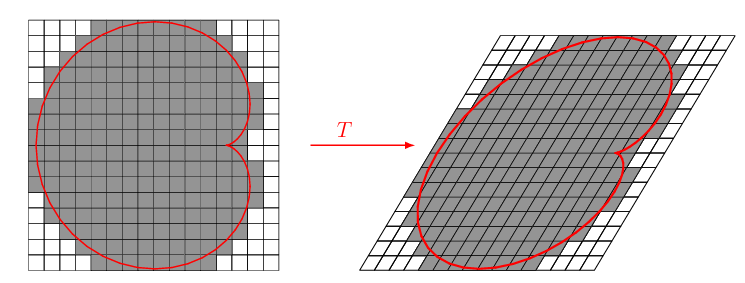
\includegraphics[width=0.6\linewidth]{Tuan2/Figures/det2.png}
\end{figure}
Vậy định thức cho một không gian ba chiều được nhìn nhận như thế nào? Vấn đề này sẽ được để lại cho độc giả với vài gợi ý nhỏ đính kèm:
\begin{enumerate}
    \item Đại lượng đặc trưng cho độ lớn của một vùng trong không gian ba chiều là gì?
    \item Hình khối tạo bởi ba vector không đồng phẳng gọi là gì?
    \item Ý nghĩa đằng sau việc một phép nhân có hướng của hai vector có thể được biểu diễn bởi một định thức; nghĩa là
    \[\mathbf{a}\times \mathbf{b}=\begin{vmatrix}
        \mathbf{e}_1 &\mathbf{e}_2 &\mathbf{e}_3\\
        a_1 & a_2 & a_3 \\
        b_1 & b_2 &b_3
    \end{vmatrix}.\]
\end{enumerate}
Các tính chất của định thức có thể được suy ra đơn thuần bằng trực giác về một phép biến đổi tuyến tính. Chẳng hạn,
\[\det(\mathbf{A}_3 \mathbf{A}_1)=\det(\mathbf{A}_2)\det(\mathbf{A}_1).\]
Nhưng vai trò của định thức là gì trong ngữ cảnh này? Mọi thứ hoá ra đều gắn với liệu định thức của một ma trận bằng hay khác 0.
Chuyện gì xảy ra khi định thức của một ma trận bằng 0? Hoặc, câu hỏi trực quan hơn là biến đổi tuyến tính của một ma trận có định thức bằng 0 mang đến một hình ảnh như thế nào. Diện tích của các hình sau biến đổi bằng 0? Đúng, nhưng 
như vậy nói lên điều gì? Rõ ràng sẽ thật tầm thường nếu ta đang đề cập tới một ma trận có toàn bộ phần tử đều bằng 0. Câu trả lời có thể được tìm thấy ở hình ảnh quen thuộc sau:
\begin{figure}[H]
    \centering
    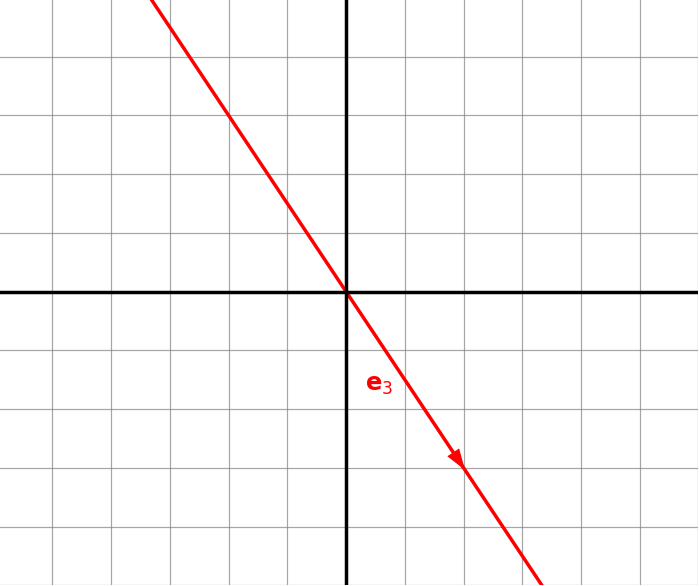
\includegraphics[width=0.5\textwidth]{Tuan2/Figures/avectoronaline.png}
\end{figure} 
Bạn còn nhớ ví dụ về hai vector \(\mathbf{e}_3\) và \(2\mathbf{e}_3\) chứ? Cho chúng vào trong một ma trận
\[\mathbf{A}=\begin{bmatrix}
    2&4\\
    -3&-6
\end{bmatrix},\] và không ngoài dự đoán \(\det(\mathbf{A})=0.\) Tất cả các vector nằm trên mặt phẳng đều bị ép vào trong đường thẳng màu đỏ, diện tích của bất cứ vùng nào sau biến đổi đều bằng 0.
Đối với một phép biến đổi như thế, ta sẽ không thể tìm được một phép biến đổi ngược lại nào đưa mọi thứ về như cũ. Nghĩa là
\[\det(\mathbf{A})=0\implies \mathbf{A}^{-1}\text{ không tồn tại}.\] Bởi, điều đó là nằm ngoài khả năng của một hàm, giống như bất cứ số nào nhân với 0 đều bằng 0, nhưng sẽ không có phép toán nào làm điều ngược lại, từ 0 lấy ra tất cả các con số khác.
Thành thử, một ma trận có thể nghịch đảo khi và chỉ khi định thức của nó khác 0. Cuối cùng, hãy nhớ rằng 
\[\mathbf{A}\mathbf{x}=\mathbf{0}\implies \det(\mathbf{A})=0.\footnote{Vì sao?}\]
\subsubsection*{Chuyển cơ sở}
\subsection{Một số ví dụ khác về không gian vector}\label{morexample}


